% ICCV 2025 Paper Template

\documentclass[10pt,twocolumn,letterpaper]{article}

%%%%%%%%% PAPER TYPE  - PLEASE UPDATE FOR FINAL VERSION
\usepackage{iccv}              % To produce the CAMERA-READY version
%\usepackage[review]{iccv}      % To produce the REVIEW version
% \usepackage[pagenumbers]{iccv} % To force page numbers, e.g. for an arXiv version

% Import additional packages in the preamble file, before hyperref
\input{preamble}

\usepackage[noend]{algpseudocode}
\usepackage{algorithm}
\usepackage{graphicx}
\usepackage{comment}
\usepackage{amsmath}

\usepackage{epsfig}
\usepackage{multirow}
\usepackage{boldline}
\usepackage{float}     % in the preamble
\usepackage{adjustbox} % already using
\usepackage{booktabs}  % for \toprule etc.
\usepackage{caption}
\usepackage{subcaption}
\usepackage{float}
\usepackage{stfloats}
\usepackage[accsupp]{axessibility}  % Improves PDF readability for those with disabilities.


% It is strongly recommended to use hyperref, especially for the review version.
% hyperref with option pagebackref eases the reviewers' job.
% Please disable hyperref *only* if you encounter grave issues, 
% e.g. with the file validation for the camera-ready version.
%
% If you comment hyperref and then uncomment it, you should delete *.aux before re-running LaTeX.
% (Or just hit 'q' on the first LaTeX run, let it finish, and you should be clear).
\definecolor{iccvblue}{rgb}{0.21,0.49,0.74}
\usepackage[pagebackref,breaklinks,colorlinks,allcolors=iccvblue]{hyperref}

%%%%%%%%% PAPER ID  - PLEASE UPDATE
\def\paperID{32} % *** Enter the Paper ID here
\def\confName{ICCVW}
\def\confYear{2025}

%%%%%%%%% TITLE - PLEASE UPDATE
\title{MK-UNet: Multi-kernel Lightweight CNN for Medical Image Segmentation}


% Md Mostafijur Rahman
% Radu Marculescu

%%%%%%%%% AUTHORS - PLEASE UPDATE
\author{Md Mostafijur Rahman\\
The University of Texas at Austin\\
Austin, Texas\\
{\tt\small mostafijur.rahman@utexas.edu}
% For a paper whose authors are all at the same institution,
% omit the following lines up until the closing ``}''.
% Additional authors and addresses can be added with ``\and'',
% just like the second author.
% To save space, use either the email address or home page, not both
\and
Radu Marculescu\\
The University of Texas at Austin\\
Austin, Texas\\
{\tt\small radum@utexas.edu}
}

\begin{document}
\maketitle


\begin{abstract}
In this paper, we introduce MK-UNet, a paradigm shift towards ultra-lightweight, multi-kernel U-shaped CNNs tailored for medical image segmentation. Central to MK-UNet is the multi-kernel depth-wise convolution block (MKDC) we design to adeptly process images through multiple kernels, while capturing complex multi-resolution spatial relationships. MK-UNet also emphasizes the images salient features through sophisticated attention mechanisms, including channel, spatial, and grouped gated attention. Our MK-UNet network, with a modest computational footprint of only 0.316M parameters and 0.314G FLOPs, represents not only a remarkably lightweight, but also significantly improved segmentation solution that provides higher accuracy over state-of-the-art (SOTA) methods across six binary medical imaging benchmarks. Specifically, MK-UNet outperforms TransUNet in DICE score with nearly 333$\times$ and 123$\times$ fewer parameters and FLOPs, respectively. Similarly, when compared against UNeXt, MK-UNet exhibits superior segmentation performance, improving the DICE score up to 6.7\% margins while operating with 4.7$\times$ fewer \#Params. Our MK-UNet also outperforms other recent lightweight networks, such as MedT, CMUNeXt, EGE-UNet, and Rolling-UNet, with much lower computational resources. This leap in performance, coupled with drastic computational gains, positions MK-UNet as an unparalleled solution for real-time, high-fidelity medical diagnostics in resource-limited settings, such as point-of-care devices. Our implementation is available at \url{https://github.com/SLDGroup/MK-UNet}.

\end{abstract}

%\vspace{-.8cm}
\section{Introduction}
\label{sec:introduction}

The field of medical image segmentation has experienced transformative growth through the development of U-shaped convolutional neural network (CNN) architectures \cite{ronneberger2015u,oktay2018attention,zhou2018unet++,fan2020pranet} such as UNet \cite{ronneberger2015u}, UNet++ \cite{zhou2018unet++}, AttnUNet \cite{oktay2018attention}, PraNet \cite{fan2020pranet}, UACANet \cite{kim2021uacanet}, and DeepLabv3+ \cite{chen2017deeplab}. These models excel at segmenting medical images, enabling precise segmentation of critical tumors, lesions, or polyps. Attention mechanisms \cite{oktay2018attention,fan2020pranet,woo2018cbam} integrated into these architectures help refine feature maps, thus enhancing pixel-level classification. However, the substantial computational demands of these models, including those with attention mechanisms, limit their applicability in resource-constrained environments such as point-of-care diagnostics.

The introduction of vision transformers \cite{chen2021transunet,cao2021swin,rahman2024g,Rahman_2023_WACV,rahman2023multi,rahman2024emcad,valanarasu2021medical}, including TransUNet \cite{chen2021transunet}, SwinUNet \cite{cao2021swin} and MedT \cite{valanarasu2021medical}, marked a shift towards leveraging self-attention to capture long-range dependencies within images for a comprehensive global view. However, transformers tend to neglect crucial local spatial relationships among pixels which are essential for precise segmentation. Moreover, transformers usually have high memory and computational demands for calculation and fusing attention with convolutional mechanisms, which limits their practical deployment. 

%UNeXt \cite{valanarasu2022unext}, a lightweight architecture, bridges this gap by combining the strengths of CNNs and multi-layer perceptron (MLP), but faces challenges in precise segmentation. 
In recent years, a good number of lightweight architectures such as UNeXt \cite{valanarasu2022unext}, CMUNeXt \cite{tang2023cmunext}, MALUNet \cite{ruan2022malunet}, EGE-UNet \cite{ruan2023ege}, and Rolling-UNet \cite{liu2024rolling}, bridge this gap by combining the strengths of CNNs and multi-layer perceptron (MLP). However, most of these architectures are designed for less complex or easy-to-segment applications such as skin lesions, breast cancer in ultrasound, and microscopic cell nuclei/structure segmentation. Consequently, these architectures show poor performance in challenging applications like polyp segmentation due to the high variability in the shape, size, and texture of polyps.


\begin{figure*}[t]
\centering
%\vspace{-.2cm}
\begin{subfigure}{.45\textwidth}
  \centering
  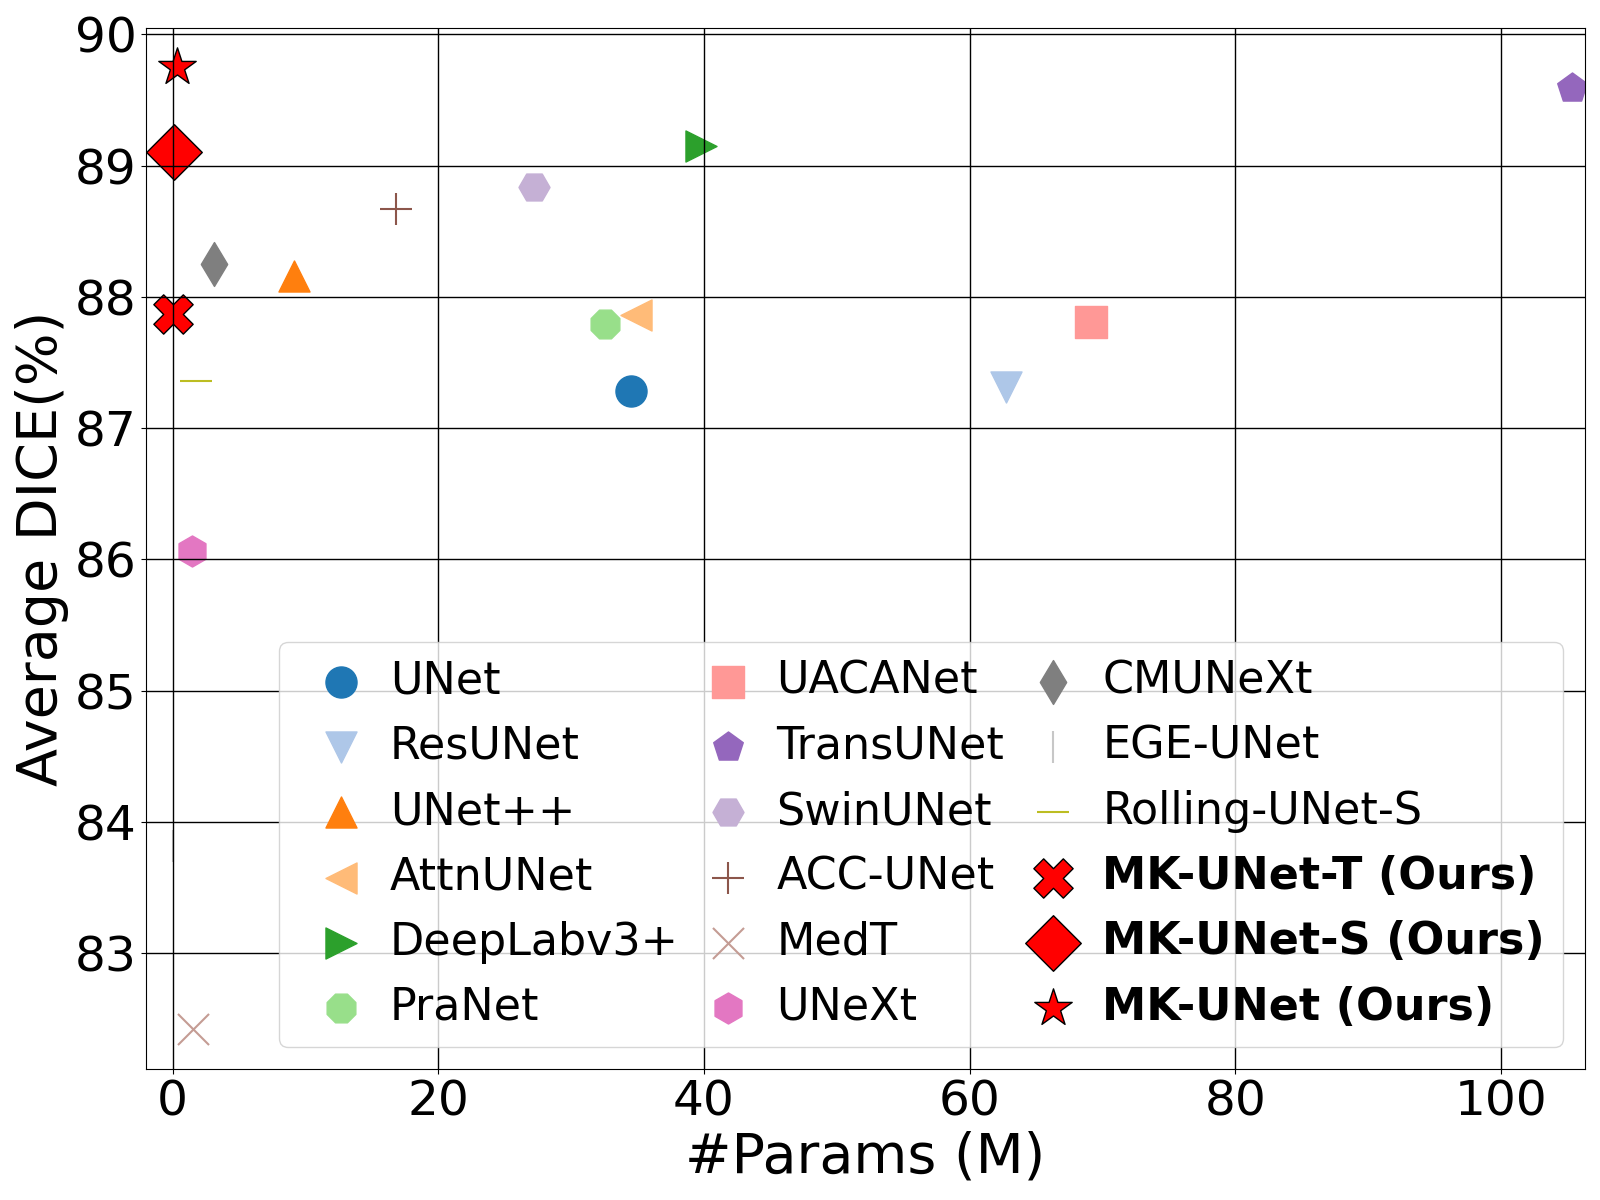
\includegraphics[width=1\linewidth]{sections/imgs/avg_dice_params_mkunet.png}
  %\vspace{-.25cm}
  \caption{Average DICE scores vs. \#Params}
  \label{fig:dice_vs_params}
\end{subfigure}%
\begin{subfigure}{.45\textwidth}
  \centering
  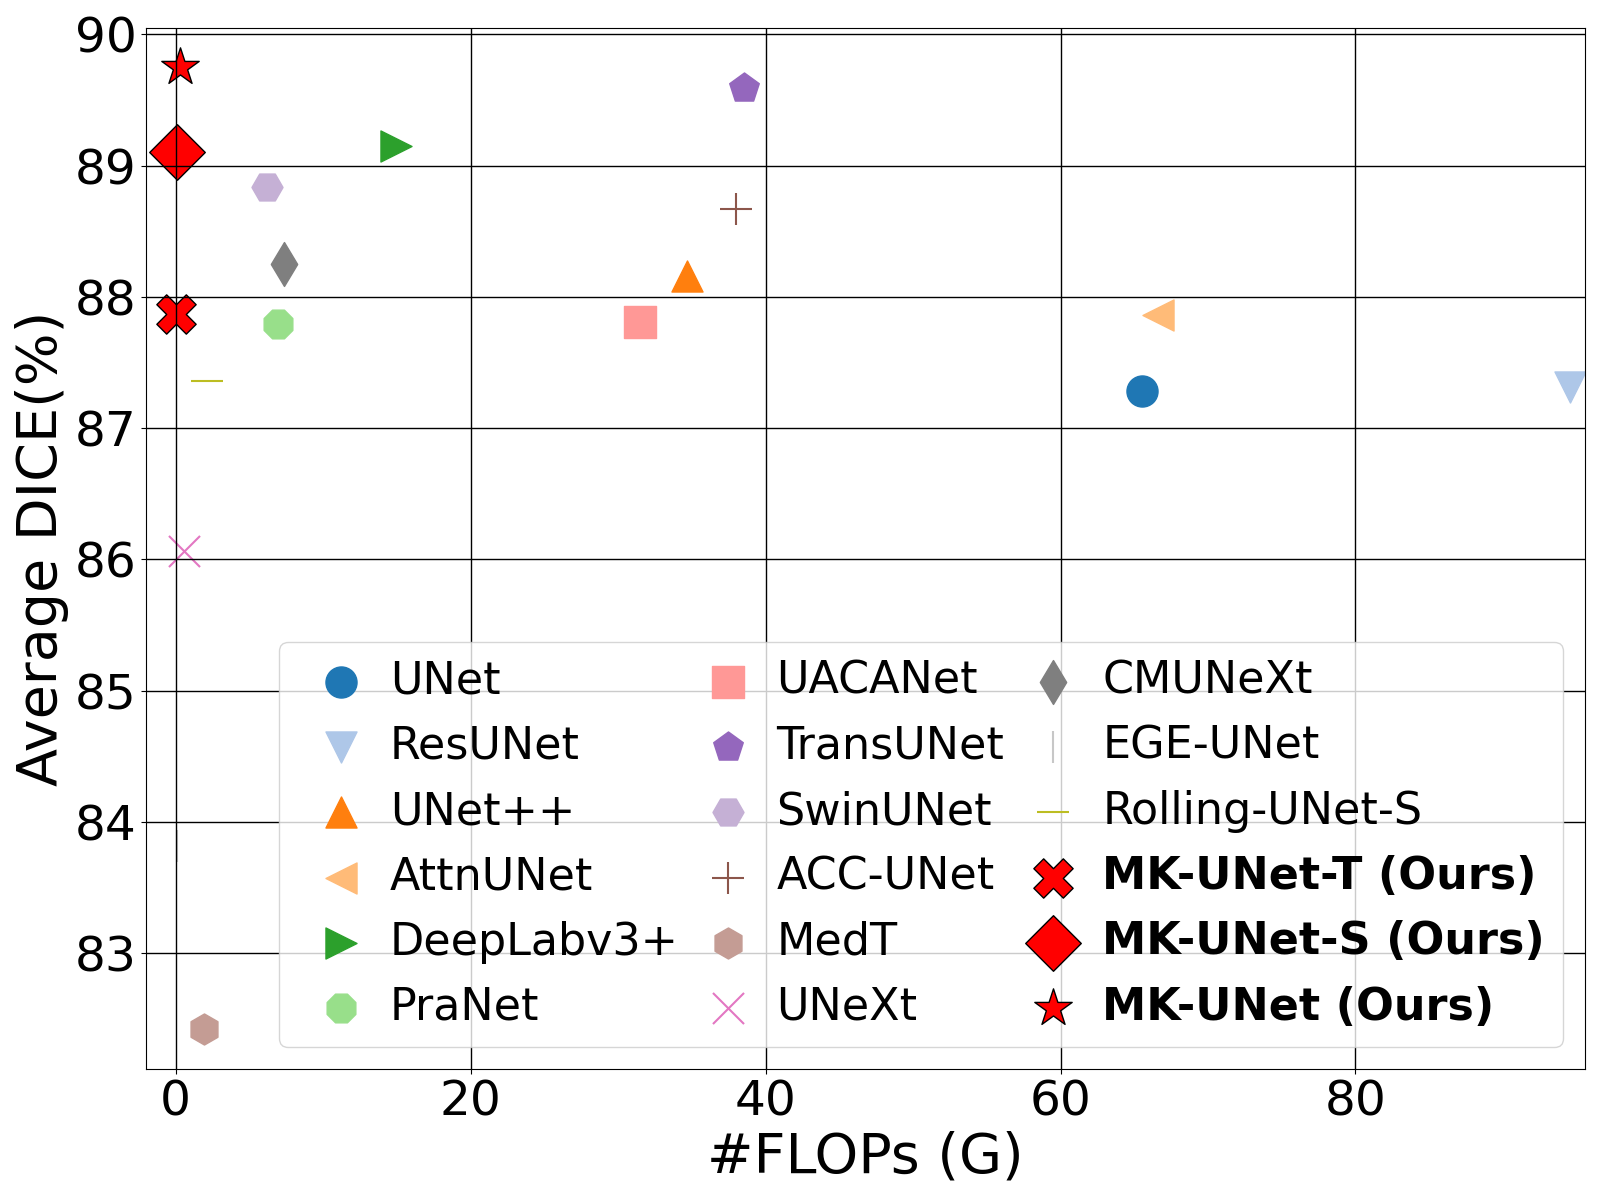
\includegraphics[width=1\linewidth]{sections/imgs/avg_dice_flops_mkunet.png}
  %\vspace{-.25cm}
  \caption{Average DICE scores vs. \#FLOPs}
  \label{fig:dice_vs_flops}
\end{subfigure}
\vspace{-.1cm}
\caption{Comparison of MK-UNet against different SOTA methods over six binary medical image segmentation datasets. As shown, our MK-UNet has the second lowest \#Params and \#FLOPs (behind EGE-UNet \cite{ruan2023ege}), yet the highest DICE scores. Though EGE-UNet has the lowest \#Params and \#FLOPs among existing methods, it has the lowest DICE score as well.}
\label{fig:dice_vs_params_flops}
\vspace{-.2cm}
\end{figure*}

%and optimization of computational resources.

To address these computational and precision challenges, we introduce MK-UNet, a significant breakthrough in image segmentation, which leverages the benefits of a multi-kernel perspective (i.e., $k_1=k_2$ or $k_1 \neq k_2$ for $k_1, k_2 \in Kernels$) and depth-wise convolutions to address the computational complexity and challenges inherent in existing CNN- and transformer-based models. Depth-wise convolutions drastically reduce the computational load, making the network more efficient without sacrificing the ability to capture detailed features within the image. Additionally, our multi-kernel property enables the model to effectively handle feature representations at \textit{same or varying} receptive fields, thus allowing for a more robust and comprehensive analysis of complex images in diverse applications. Moreover, by incorporating sophisticated convolutional multi-focal (channel and spatial) attention mechanisms \textit{only} in our decoder further refines the feature maps by capturing the image salient features. We note that our network is effective for segmentation in both scenarios, whether the regions of interest vary significantly in size and shape or remain relatively uniform. By integrating these new ideas, MK-UNet achieves a fine balance between computational efficiency and segmentation accuracy, thus offering an ultra-lightweight model that not only surpasses the performance of heavyweight counterparts (in DICE scores), but it does so with significantly fewer \#Params and \#FLOPs. Our contributions are as follows:

\begin{itemize}
%\vspace{-.2cm}
    \item \textbf{New Lightweight Multi-kernel UNet:} We propose a new end-to-end U-shaped network, MK-UNet, for medical image segmentation, which encodes an image using lightweight multi-kernel convolutions to capture multi-resolution spatial representations. MK-UNet also progressively refines the multi-resolution spatial representations using multi-kernel convolutional attention. Of note, our MK-UNet-T (tiny) has only 0.027M and 0.062G \#Params and \#FLOPs, respectively, yet provides SOTA performance. Moreover, MK-UNet (standard) has only 0.316M \#Params and 0.314G \#FLOPs. The extremely low model size (\#Params) and computations (\#FLOPs) make our MK-UNet easy to deploy in point-of-care diagnostics or resource-constraint environments (e.g., mobile or edge devices).
    \item \textbf{Lightweight Multi-kernel Inverted Residual:} We introduce MKIR, a new Multi-Kernel Inverted Residual block that performs depth-wise convolutions with multiple kernels (i.e., $k_1=k_2$ or $k_1 \neq k_2$, for $k_1, k_2 \in Kernels$). Our encoder extracts features using the MKIR block; this choice is motivated by the need to efficiently process and encode diverse and complex structures in medical images, thus providing a rich representation with minimal computational costs.
    \item \textbf{Lightweight Multi-kernel Inverted Residual Attention:} We propose Multi-Kernel Inverted Residual Attention (MKIRA), a new block to refine and enhance multi-scale salient features by suppressing irrelevant regions. In our decoder, MKIRA enhances features discrimination by focusing on key feature channels and highlighting the important spatial regions in an image. This ensures that the decoder can reconstruct precise and accurate segmentation maps by focusing only on the most critical aspects of the encoded features. 
    %\item \textbf{Lightweight Grouped Attention Gate:} We introduce a new grouped attention gate to combine refined features with skip connections. By using $3\times3$ group convolutions instead of point-wise convolutions, our attention gate captures salient features in a larger local context with less computation.
    \item \textbf{Improved Performance across Various Tasks and Benchmarks:} We empirically show that MK-UNet significantly improves the performance of medical image segmentation compared to SOTA methods with a significantly lower computational cost (as shown in Fig. \ref{fig:dice_vs_params_flops}) on six binary medical image segmentation benchmarks that belong to four different tasks.
\end{itemize}

The remaining of this paper is organized as follows: Section \ref{sec:method} describes the proposed method. Section \ref{sec:experiments} explains our experimental setup and results on six medical image segmentation benchmarks. Section \ref{sec:ablation_study} covers different ablation experiments. Lastly, Section \ref{sec:conclusion} concludes the paper. 
%-------------------------------------------------------------------------



\section{Related Work}
\label{sec:related_work}

%Over the years, deep learning has revolutionized the medical image segmentation domain by providing SOTA performance on a wide range of tasks. This section reviews the advancements in CNN-based, Vision Transformer-based, and Lightweight models in medical image segmentation, that are relevant to our proposed MK-UNet.

\subsection{Convolutional Neural Networks (CNNs)}
The advent of CNNs marks a significant shift in medical image segmentation \cite{ronneberger2015u, oktay2018attention, zhou2018unet++, fan2020pranet, kim2021uacanet, chen2017deeplab}. Pioneering work such as Fully Convolutional Networks (FCNs) \cite{long2015fully} laid the foundation for end-to-end segmentation models. FCNs replace fully connected layers with convolutional layers, thus enabling pixel-wise predictions and efficient learning of spatial hierarchies in images. U-Net \cite{ronneberger2015u} became a cornerstone in medical image segmentation due to its encoder-decoder architecture with skip connections. This design effectively combines high-resolution features from the encoder with context information from the decoder, hence leading to precise segmentation even with limited training data. The sophisticated design of U-shaped architecture for pixel-level segmentation tasks motivates us to choose the U-shaped design in our proposed network.

U-Net's success has inspired numerous variants and improvements. Inspired by residual learning in ResNet \cite{he2016deep}, ResUNet \cite{zhang2018road} uses residual blocks to facilitate gradient flow and improve convergence, addressing the vanishing gradient problem in deep networks. Zhou et al.\cite{zhou2018unet++} introduce UNet++, which uses dense nested skip connections to further enhance the feature propagation and improve the segmentation accuracy. AttnUNet \cite{oktay2018attention} incorporates attention mechanisms to focus on relevant regions in the feature maps, improving segmentation performance by suppressing irrelevant background noise. Fan et al. \cite{fan2020pranet} introduce PraNet for precise polyp segmentation that employs parallel reverse attention and edge-guidance to refine segmentation boundaries. UACANet \cite{kim2021uacanet} uses uncertainty-aware mechanisms to improve the reliability and robustness of segmentation outcomes. DeepLabv3+ \cite{chen2017deeplab} integrates atrous convolutions and spatial pyramid pooling to capture multi-scale context information. ACC-UNet \cite{ibtehaz2023acc} employs adaptive context capture mechanisms to dynamically adjust the receptive fields based on the input image.

\subsection{Vision Transformers}
Vision Transformers (ViTs) \cite{dosovitskiy2020image, liu2021swin} have emerged as a powerful alternative to CNNs, offering a new paradigm for medical image analysis tasks by leveraging the self-attention mechanism \cite{chen2021transunet, cao2021swin, rahman2024emcad, Rahman_2023_WACV, rahman2023multi, rahman2024g, valanarasu2021medical}. By combining the strengths of CNNs for local feature extraction and Transformers for capturing long-range dependencies, TransUNet \cite{chen2021transunet} achieves superior performance in medical image segmentation. SwinUNet \cite{cao2021swin} is introduced based on the Swin Transformer \cite{liu2021swin} architecture, which utilizes shifted windows to achieve hierarchical feature representation, enabling efficient computation. MedT \cite{valanarasu2021medical}, a lightweight Transformer model specifically designed for medical image segmentation, which employs gated axial attention mechanisms to focus on relevant regions and reduce computational complexity. Rahman et al. introduce CASCADE \cite{Rahman_2023_WACV}, a cascaded-attention decoding network using standard convolutions. Recently, EMCAD \cite{rahman2024emcad} introduces a depthwise convolutions-based multi-scale decoder. Although, CASCADE and EMCAD perform well in medical image segmentation, their segmentation accuracy and computational complexity solely depend on the strength and complexity of the exiting pretrained transformer encoder they use, thus making them less suitable for resource-constrained settings. In contrast, we propose to design an extremely efficient (ultra-lightweight) end-to-end (both encoder and decoder) architecture using the multi-kernel trick (where, $k_1=k_2$ or $k_1 \neq k_2$ for $k_1, k_2 \in Kernels$) with depthwise convolutions.

\subsection{Lightweight CNNs}
Recent efforts have focused on making CNNs more efficient for real-time and resource-constrained environments. MobileNets \cite{howard2017mobilenets} and EfficientNets \cite{tan2019efficientnet} introduce depthwise separable convolutions and compound scaling, respectively, to create lightweight models with competitive performance. Additionally, several novel lightweight architectures have been developed to further enhance the efficiency of medical image segmentation \cite{valanarasu2022unext, tang2023cmunext, ruan2023ege, liu2024rolling}. UNeXt \cite{valanarasu2022unext} uses hybrid convolutional and transformer blocks to capture local and global features efficiently, improving segmentation accuracy while maintaining computational efficiency. CMUNeXt \cite{tang2023cmunext} combines convolutional and multi-scale features to enhance segmentation performance. EGE-UNet \cite{ruan2023ege} integrates edge-guided mechanisms to refine segmentation boundaries. Rolling-UNet \cite{liu2024rolling} incorporates rolling convolutional blocks to enhance the model's ability to capture long-range dependencies.
\begin{figure*}[t]
%\vspace{-.1cm}
\centering
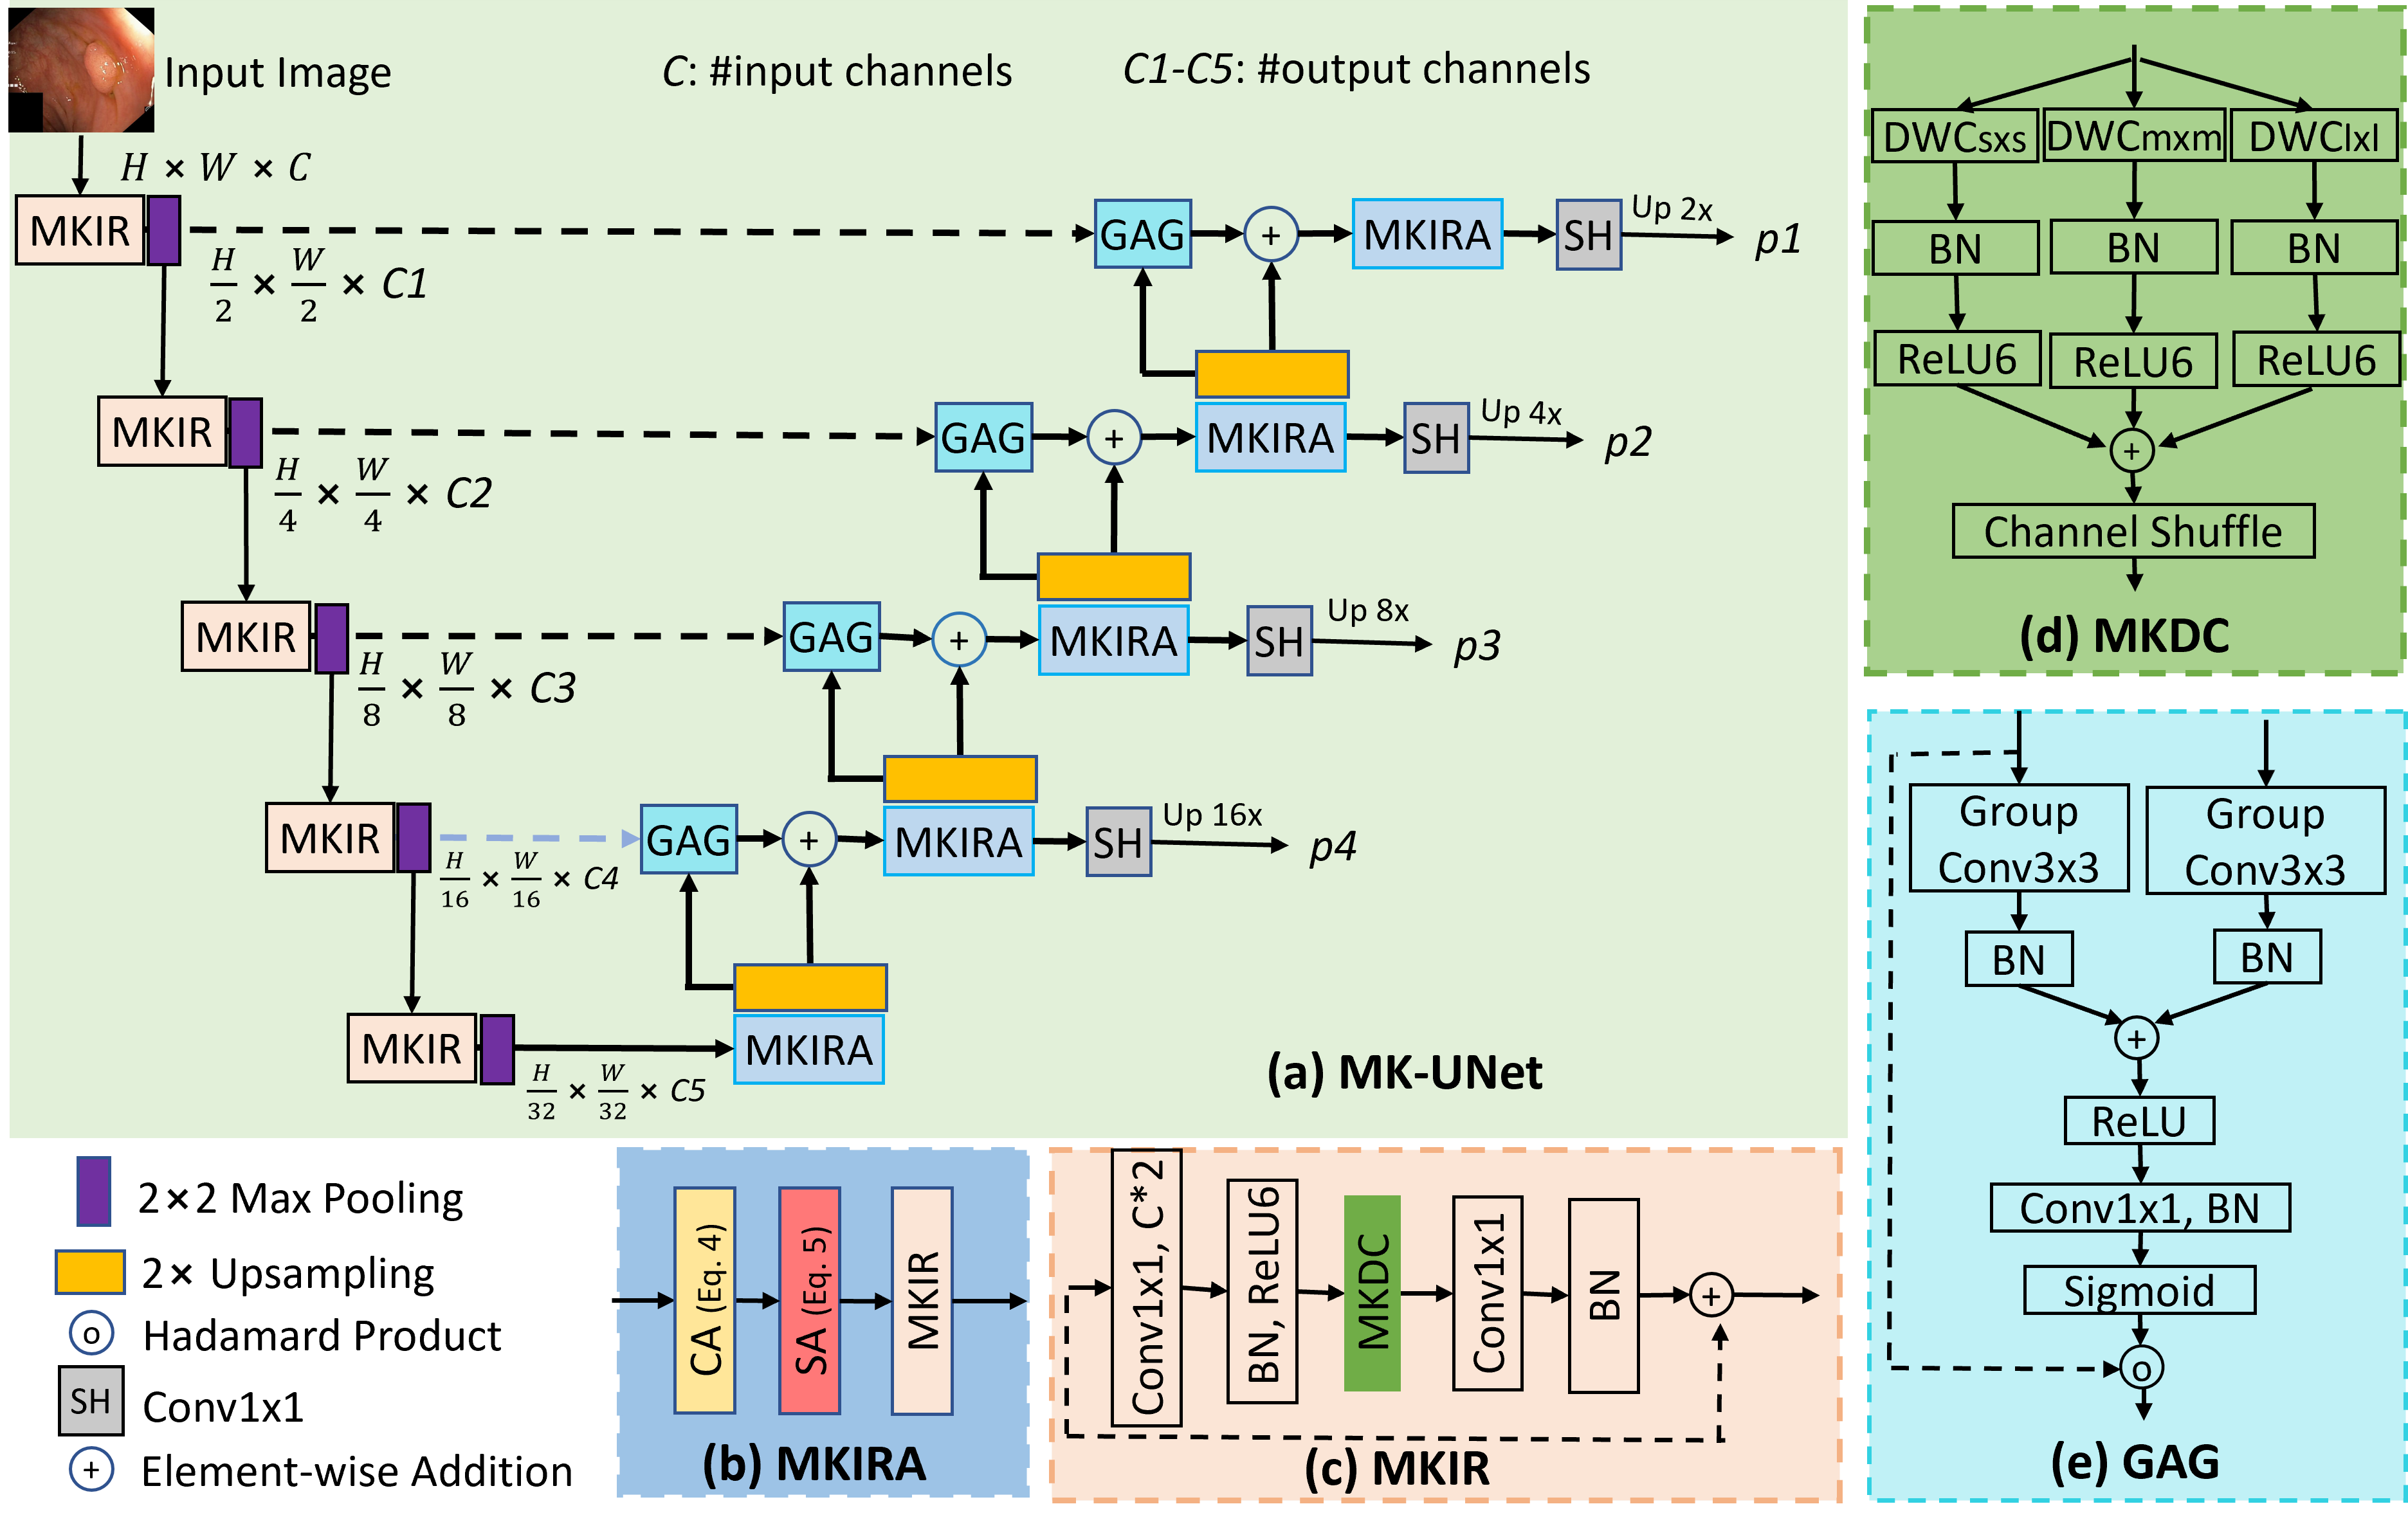
\includegraphics[width=0.88\textwidth]{sections/imgs/mk_unet_architecture.png}
\vspace{-.2cm}
\caption{The proposed network diagram. (a) Five-stage MK-UNet network (b) Multi-kernel inverted residual attention (MKIRA), (c) Multi-kernel inverted residual (MKIR), (d) Multi-kernel (parallel) depth-wise convolution (MKDC), (e) Grouped attention gate (GAG). p1, p2, p3, and p4 are output segmentation maps. \textbf{Note}: Channel attention (CA), Spatial attention (SA).}
\label{fig:architecture}
\vspace{-.2cm}
\end{figure*}

\section{Method}
\label{sec:method}
We describe next our core building blocks. Then, we introduce our MK-UNet architecture by integrating these blocks into the baseline UNeXt \cite{valanarasu2022unext} (Fig. \ref{fig:architecture}a in green box). %Different components are described below.

\subsection{Multi-kernel Inverted Residual (MKIR)} 
We first introduce the multi-kernel inverted residual ($MKIR$) block to generate and refine feature maps (Fig. \ref{fig:architecture}c). By utilizing multiple (same or different) kernel sizes, $MKIR$ allows for better understanding of both fine-grained details and broader contexts, thereby enabling a comprehensive representation of the input. As shown in Fig. \ref{fig:architecture}c, the process begins by expanding the \#channels (i.e., expansion\_factor = 2) through point-wise convolution $PWC_1$, batch normalization $BN$ \cite{ioffe2015batch}, and $ReLU6$ activation \cite{krizhevsky2010convolutional}. This is followed by multi-kernel depth-wise convolution $MKDC$ for capturing application-specific complex spatial contexts. A subsequent point-wise convolution $PWC_2$ and $BN$ restore the original \#channels. The MKIR (Eq. \ref{eq:mkir}) significantly reduces the computational cost while ensuring rich feature representation: %\scriptsize
\begin{equation}
%\vspace{-.05cm}
\scalebox{0.75}{\(
    MKIR(x) = BN(PWC_2(MKDC(ReLU6(BN(PWC_1(x))))))
\)}
%\vspace{-.05cm}
    \label{eq:mkir}
\end{equation}
%\normalsize
where $MKDC$ for multiple kernels ($K$) is defined in Eq. \ref{eq:mkdc} and Fig. \ref{fig:architecture}d: %\vspace{-.05cm}
\begin{equation}
    \scalebox{0.9}{\( 
    MKDC(x) = CS(\sum_{k \in K} DWCB_{k}(x))
    \)}
    %\vspace{-.05cm}
    \label{eq:mkdc}
\end{equation}
where $DWCB_{k}(x) = ReLU6(BN(DWC_{k}(x)))$. Here, $DWC_{k}$(.) is a depth-wise convolution with the kernel $k\times k$. To address the channel independence in depth-wise convolution, a channel shuffle ($CS$) is used to ensure the inter-channel information flow. Our $MKDC(.)$ differs from $MSCB$ (in EMCAD \cite{rahman2024emcad}) in their core theoretical concepts. Our multi-kernel trick supports both $k_1=k_2$ (same-size kernels) and $k_1 \neq k_2$ (different-size kernels) for $k_1, k_2 \in K$ versus conventional multi-scale (only $k_1 \neq k_2$) designs \cite{rahman2024emcad, lin2023scale, seo2022spatial}, thus allowing adaptable context extraction.
This conceptual distinction allows MK-UNet to adapt kernel sizes based on application-specific needs (e.g., large kernels for large objects, small kernels for small objects, or mixed for both objects segmentation).  %Additionally, our sequential $MKDC$(.) uses the recursively updated input $x$, where the input $x$ is residually connected to the previous $DWCB_{ks}$(.) for better regularization as in Eq. \ref{eq:msdc_sequential}: 
%\vspace{-.2cm}
%\begin{equation}
%    x = x + DWCB_{ks}(x)
%    \vspace{-.2cm}
%    \label{eq:msdc_sequential}
%\end{equation}
%\vspace{-.4cm}

%\vspace{-.4cm}
\subsection{Multi-kernel Inverted Residual Attention (MKIRA)}
We present a lightweight multi-kernel inverted residual attention, MKIRA, to refine the feature maps ($x$). MKIRA uses channel attention ($CA$) \cite{hu2018squeeze} to focus on relevant channels, a spatial attention ($SA$) \cite{chen2017sca} to capture the local context, and a multi-kernel inverted residual ($MKIR$) to enrich the feature maps while capturing contextual relationships. The $MKIRA$ (Fig. \ref{fig:architecture}b) is given in Eq. \ref{eq:mkira}: 
%\vspace{-.25cm}
\begin{equation}
    MKIRA(x) = MKIR(SA(CA(x)))
    %\vspace{-.2cm}
    \label{eq:mkira}
\end{equation}
%where $x$ is the input tensor. Employing depth-wise convolution with multiple kernels, MKIRA achieves significant computational efficiency.

%\vspace{-.4cm}

%\vspace{-.8cm}
\noindent \textit{Channel Attention (CA):} 
%We use channel attention block to assign different levels of importance to each channel, thus emphasizing more relevant features while suppressing less useful ones. Basically, the CA identifies \textit{which feature maps} to focus on (and then refine them). Following \cite{woo2018cbam}, in CA, we first apply the adaptive maximum pooling ($P_m$(·)) and adaptive average pooling ($P_a$(·)) to the spatial dimensions (i.e., height and width) to extract the most significant feature of the entire feature map per channel. Then, for each pooled feature map, we reduce the number of channels $r=16$ times separately using a point-wise convolution ($C_1$(·)) followed by a ReLU activation ($R$). Afterward, we recover the original channels using another point-wise convolution ($C_2$(·)). We then add both recovered feature maps and apply Sigmoid ($\sigma$) activation to estimate attention weights. Finally, we incorporate these weights to input $x$ using the Hadamard product ($\circledast$). The $CA$(·) (Fig. \ref{fig:architecture}(f)) is defined using Eq. \ref{eq:ca}: 
We use $CA$ \cite{hu2018squeeze} to enhance relevant features by applying adaptive max ($AMP$) and average pooling ($AAP$) to condense the spatial information \cite{Rahman_2023_WACV}; this is followed by channel reduction ($r = 16$) through point-wise convolution $PWC_1$ with $ReLU$ ($R$) activation \cite{nair2010rectified} and expansion through $PWC_2$. The $Sigmoid$ ($\sigma$) activation generates attention weights, which are then applied to the input via the Hadamard product ($\circledast$), while focusing on crucial feature maps. The $CA$ is defined in Eq. \ref{eq:ca}:%\vspace{-.2cm}
 %\small 
 \begin{equation}
 \scalebox{0.62}{\( CA(x)=\sigma(PWC_2(R(PWC_1(AMP(x))))+PWC_2(R(PWC_1(AAP(x))))) \circledast x
 \)}
 %\vspace{-.25cm}
    \label{eq:ca}
\end{equation}
%\normalsize
%where $\circledast$ is the Hadamard product. 
%$\sigma$(·) is the Sigmoid activation. $P_m$(·) and $P_a$(·) denote adaptive maximum pooling and adaptive average pooling, respectively. $C_1$(·) is a convolutional layer with $1 \times 1$ kernel size to reduce the channel dimension 16 times. $R$ is a ReLU activation layer and $C_2$(·) is another convolutional layer to recover the original channel dimension. 
%\vspace{-.8cm}

\noindent \textit{Spatial Attention (SA):} 
%We use spatial attention to mimic the attentional processes of the human brain by focusing on specific parts of an input image. Basically, the SA determines \textit{where} to focus in a feature map; then it enhances those features. This process enhances the model's ability to recognize and respond to relevant spatial features, which is crucial for image segmentation where the context and location of objects significantly influence the output. In SA, we first pool maximum ($Channel_{max}$(·)) and average ($Channel_{avg}$(·)) values along the channel dimension to pay attention to local features. Then, we use a large kernel (i.e., $7 \times 7$ as in \cite{dong2021polyp}) convolution layer $LKC$(.) to enhance local contextual relationships among features. Afterward, we apply the Sigmoid activation to calculate attention weights. Finally, we feed these weights to the input $x$ (using Hadamard product ($\circledast$) to attend information in a more targeted way. The $SA$(.) (Fig. \ref{fig:architecture}(g)) is defined using Eq. \ref{eq:sa}:
We use $SA$ \cite{chen2017sca} to focus on specific image regions to highlight key features, crucial for accurate segmentation. The $SA$ aggregates maximum ($Ch_{max}$) and average ($Ch_{avg}$) channel values to highlight local details, then it employs a large-kernel ($7 \times 7$) convolution ($LKC$) to strengthen the contextual connections. The $Sigmoid$ ($\sigma$) activation derives attention weights, applied to the input $x$ via the Hadamard product ($\circledast$), ensuring targeted refinement. The $SA$ is derived in Eq. \ref{eq:sa}:
%\vspace{-.2cm}
\begin{equation}
    SA(x) = \sigma(LKC([Ch_{max}(x), Ch_{avg}(x)])) \circledast x
    %\vspace{-0.2cm}
    \label{eq:sa}
\end{equation}
\normalsize

%\vspace{-.5cm}
\subsection{Grouped attention gate (GAG)}
We use a grouped attention gate ($GAG$, Fig. \ref{fig:architecture}e) that mixes the feature maps with the attention coefficients for enhancing the relevant features and suppressing the irrelevant ones. By utilizing a gating signal from higher-resolution features, $GAG$ directs the information flow, thus improving medical image segmentation accuracy. Unlike Attention UNet \cite{oktay2018attention}, which processes signals with $1\times1$ convolution, our method applies $3\times3$ group convolutions ($GC$) to both gating ($g$) and input ($x$) feature maps separately \cite{rahman2024emcad}. After convolution, the features undergo batch normalization ($BN$) and get combined via addition, followed by $ReLU$ ($R$) activation. Subsequently, a $1\times1$ convolution and batch normalization ($BN$) produce a unified feature map which, after the $Sigmoid$ activation ($\sigma$), generates the attention coefficients. These coefficients adjust the input feature $x$, and create an attention-enhanced output. $GAG$ is defined in Eq.s \ref{eq:ags_1}:% and \ref{eq:ags_2}:
%\vspace{-.1cm}
\begin{equation}
\scalebox{0.7}{\(
   GAG(g, x) = x \circledast \sigma(BN(Conv(R(BN(GC_g(g) + BN(GC_x(x)))))))))%q_{gag}(g, x))))
   \)}
   %\vspace{-.3cm}
    \label{eq:ags_1}
\end{equation} 
%\begin{equation}
%\scalebox{0.9}{\(
%    q_{gag}(g, x) = ReLU(BatchNorm(GroupConv_g(g) + BatchNorm(GroupConv_x(x)))))
%    \)}
%    %\vspace{-.25cm}
%    \label{eq:ags_2}
%\end{equation}
%\vspace{-.3cm}
%The $3\times3$ group convolutions in our GAG enhance the spatial context with lower computational cost, thus setting a new standard for gated feature map combination.

%Our implementation of $3\times3$ kernel group convolutions within $q_{gag}$(.) allows the GAG to access broader spatial contexts while minimizing computational demands, setting a new standard for feature map combination and attention gating in neural networks, particularly for enhancing medical imaging performance.

%\vspace{-.4cm}

%\subsection{Segmentation head (SH)}
%We use segmentation heads to produce the segmentation outputs from the refined feature maps of four stages of the decoder. The SH layer applies a $1\times1$ convolution $Conv_{1\times1}$(·) to the refined feature maps having $ch_i$ channels ($ch_i$ is the \#channels in the feature map of stage $i$) and produces output with \#channels equal to \#classes in target dataset for multi-class but $1$ channel for binary segmentation. The $SH$(·) is formulated as in Eq. \ref{eq:seg_head}:
%\begin{equation}
%    SH(x) = Conv_{1\times1}(x)
%    %\vspace{-0.1cm}
%    \label{eq:seg_head}
%\end{equation}

%\vspace{-.5cm}
\subsection{Multi-kernel UNet (MK-UNet)}
%Existing transformer-based models have limited (local) contextual information processing ability among pixels. As a result, the transformer-based model faces difficulties in locating the more discriminating local features. To address this issue, some works \cite{dong2021polyp,Rahman_2023_WACV, rahman2023multi} utilize computationally expensive 2D convolution blocks in the decoder. Although the convolution block helps to incorporate the local information, it results in long-range attention deficits. To overcome this problem, we propose a new cascaded graph convolutional decoder, G-CASCADE, for pyramid encoders.
%In this part, we introduce our multi-kernel UNet to process an image through multiple stages and produce high-resolution segmentation maps. As shown in Fig. \ref{fig:architecture}(a), MK-UNet has five encoder stages and five decoder stages. In each encoder stage, a multi-kernel inverted residual (MKIR) block is used to produce $C_i$ feature maps. Afterward, a Max Pooling layer is used to downsample the input by preserving important information. The feature map generated by the fifth stage of the encoder is fed into a multi-kernel inverted residual attention (MKIRA) block at the first stage of the decoder to robustly enhance the feature maps. Afterward, the enhanced feature map is up-sampled $2\times$ using Bilinear interpolation to feed into second stage of the decoder. Last four stages of the decoder first use a grouped attention gate (GAG) to refine feature maps fusing with the skip connection via gated attention mechanism. Then, refine the feature map using MKIRA block and up-sample the feature map $2\times$ to match with next-satge skip connections. Four segmentation heads (SHs) are used to produce segmentation outputs from last four stages of decoder. Different modules of our network are described next.
Our MK-UNet employs a multi-kernel approach across five encoding and decoding stages to generate high-resolution segmentation maps, as depicted in Fig. \ref{fig:architecture}a. Each encoding stage uses a multi-kernel inverted residual (MKIR) block to produce $C_i$ feature maps, followed by max pooling for downsampling while retaining crucial information. The output from the final encoding stage passes through a multi-kernel inverted residual attention (MKIRA) block in the decoder's initial stage, significantly refining the feature maps. These are then upsampled using bilinear interpolation for subsequent decoding stages. Decoder stages integrate skip-connections with refined features using a grouped attention gate (GAG) followed by additive aggregation. The resultant feature maps are refined through the MKIRA block and up-sampled (only bilinear $2\times$, no convolutions) to align with the later stages. 

The segmentation heads (SHs) at the last four stages output the segmentation maps $p_4$, $p_3$, $p_2$, and $p_1$. We consider the feature map $p_1$ as final prediction and obtain the final segmentation output by employing a $Sigmoid$ for binary segmentation or a $Softmax$ activation for multi-class segmentation. We optimize the loss of only final prediction $p_1$ for all binary segmentation tasks. However, we recommend using deep supervision for multi-class segmentation.

%\vspace{-.4cm}
%\subsection{Loss aggregation and output generation}

%\vspace{-.1cm}
%\textbf{Multi-stage loss aggregation:}
%We get four output segmentation maps $p_1$, $p_2$, $p_3$, and $p_4$ from the four prediction heads for the four stages of our EMCAD decoder. 
%Our MK-UNet's four segmentation heads (SHs) produce four prediction maps $p_1$, $p_2$, $p_3$, and $p_4$ across its stages. We optimize the loss of only final prediction map $p_4$ for all binary segmentation. %We adopt a combinatorial approach to loss combination called MUTATION, inspired by the work of MERIT \cite{rahman2023multi} for multi-class segmentation. This involves calculating the loss for all possible combinations of predictions derived from $4$ heads, totaling $2^4-1=15$ unique predictions, and then summing these losses. We focus on minimizing this cumulative combinatorial loss during the training process.
%For binary segmentation, 
%While for multi-class segmentation, we optimize the additive loss like \cite{Rahman_2023_WACV} with an additional term $\mathcal{L}_{p_1 + p_2 + p_3 + p_4}$ as in Eq. \ref{eq:add_loss}: \vspace{-0.2cm}
%\begin{equation}
%\scalebox{0.95}{\(
%   \mathcal{L}_{total} = \mathcal{L}_{p_1} + \mathcal{L}_{p_2} + \mathcal{L}_{p_3} + \mathcal{L}_{p_4} + \mathcal{L}_{p_1 + p_2 + p_3 + p_4}
%\)}
%\vspace{-0.2cm}
%\label{eq:add_loss}
%\end{equation}
%where $\mathcal{L}_{p_1}$, $\mathcal{L}_{p_2}$, $\mathcal{L}_{p_3}$, and $\mathcal{L}_{p_4}$ are the losses of different stages prediction maps. 
    

%Following MERIT \cite{rahman2023multi}, we use the combinatorial loss aggregation strategy, MUTATION in all our experiments. Therefore, we compute the loss for $2^n-1$ combinatorial predictions synthesized from $n$ heads separately and then do a summation of them. We optimize this additive combinatorial loss during training.

%\noindent \textbf{Output segmentation map generation:} %We derive the final segmentation output by summing up the weighted contributions of each segmentation map as in Eq. \ref{eq:output_aggregation}:
%\begin{equation}
%    seg\_map = \alpha p_1 + \beta p_2 + \gamma p_3 + \zeta p_4
%    \vspace{-0.1cm}
%\label{eq:output_aggregation}
%\end{equation}
%where $\alpha$, $\beta$, $\gamma$, and $\zeta$ represent the weights assigned to each prediction head. For all experiments, these weights are uniformly set to $1.0$. 
%We consider the feature map $p_4$ from fifth stage as final prediction and obtain the final segmentation output by employing a Sigmoid function for binary segmentation or a Softmax function for multi-class segmentation.
%\vspace{-.2cm}
\section{Experiments and Results}
\label{sec:experiments}
%\vspace{-.2cm}
\subsection{Datasets}
\label{assec:Datasets}
We evaluate the MK-UNet's efficacy across six datasets covering four segmentation tasks, including breast cancer (BUSI \cite{al2020dataset}, 647 images: 437 benign and 210 malignant), polyp (ClinicDB \cite{bernal2015wm} with 612 images, and ColonDB \cite{vazquez2017benchmark} with 379 images), skin lesion (ISIC18 \cite{codella2019skin}, 2,594 images), and cell nuclei/structure segmentation (DSB18 \cite{caicedo2019nucleus} with 670 images, and EM \cite{cardona2010integrated} with 30 images). These datasets, collected from various imaging centers, offer a broad diversity in image characteristics, ensuring a comprehensive evaluation. An 80:10:10 train-val-test split was applied across all datasets and the DICE score of testset is reported.

%We evaluate the performance of our MK-UNet network, we conduct experiments across six datasets that belong to four medical image segmentation tasks. Specifically, we use BUSI \cite{al2020dataset} dataset for breast cancer segmentation. Following \cite{valanarasu2022unext}, we use 647 (437 benign and 210 malignant) images from this dataset. Besides, we use two polyp segmentation datasets: ClinicDB \cite{bernal2015wm} (612 images), and ColonDB \cite{vazquez2017benchmark} (379 images). These datasets contain images from different imaging centers/clinics, having greater diversity in image nature as well as size and shape of polyps. We consider ISIC18 \cite{codella2019skin} dataset (2,594 images) for skin lesion segmentation. DSB18 \cite{caicedo2019nucleus} (670 images) and EM \cite{cardona2010integrated} (30 images) datasets of biological imaging are used for cell nuclei/structure segmentation. We follow a train-val-test split of 80:10:10 in all the datasets.

%\vspace{-0.4cm}
\subsection{Implementation details}
\label{ssec:impl_details}
%We implement our network and conduct experiments using Pytorch 1.11.0 on a single NVIDIA RTX A6000 GPU with 48GB of memory. In the MKDC of our network, we set the multi-scale kernels $[1,3,5]$ through an ablation study. We use the parallel arrangement of depth-wise convolutions and the MK-UNet network with $[16,32,64,96,160]$ channels default in all experiments unless otherwise mentioned. Our models are trained using the AdamW optimizer \cite{loshchilov2017decoupled} with a learning rate and weight decay of $1e-4$. We train for 200 epochs with a batch size of 16, saving the best model based on the DICE score. We resize images to $256\times256$ for ISIC18 \cite{codella2018skin}, BUSI \cite{al2020dataset}, EM \cite{cardona2010integrated}, and DSB18 \cite{caicedo2019nucleus}. For ClinicDB \cite{bernal2015wm} and ColonDB \cite{vazquez2017benchmark}, images are resized to $352\times352$. We use a multi-scale \{0.75, 1.0, 1.25\} training strategy with a gradient clip limit of 0.5. We do not use any augmentation and optimize a combined weighted BinaryCrossEntropy (BCE) and weighted IoU loss function. 

Our networks are developed and evaluated using Pytorch 1.11.0, operating on a single NVIDIA RTX A6000 GPU equipped with 48GB of RAM.  We utilize multi-scale kernels $[1,3,5]$ within our MKDC, based on an ablation study. The architecture employs a series of parallel depth-wise convolutions in the MK-UNet network, standardizing on channel configurations of $[16,32,64,96,160]$ across all experiments, unless specified otherwise. Model optimization is achieved via the AdamW \cite{loshchilov2017decoupled} optimizer with both learning rate and weight decay set to $1e-4$. Training spans over 200 epochs with batches of 16, during which we save the model achieving the highest DICE score. 

Image dimensions are set to $256\times256$ pixels for BUSI \cite{al2020dataset}, ISIC18 \cite{codella2018skin}, EM \cite{cardona2010integrated}, and DSB18 \cite{caicedo2019nucleus} datasets, while for ClinicDB \cite{bernal2015wm} and ColonDB \cite{vazquez2017benchmark}, the resolution is adjusted to $352\times352$ pixels. We utilize a multi-scale training approach, with scales of \{0.75, 1.0, 1.25\}, and enforce gradient clipping at 0.5. We do not apply any form of augmentation and use a hybrid loss function that combines (1:1) weighted BinaryCrossEntropy (BCE) with a weighted Intersection over Union (IoU) loss.

%Following \cite{rahman2023cascade}, we resize images to $224\times224$, employ random rotation and flipping as data augmentation, and optimize the combined Cross-entropy (0.3) and DICE (0.7) loss for Synapse multi-organ and ACDC datasets. 
%We use a batch size of 6 and train each model for maximum of 300 epochs. We use the input resolution of $224 \times 224$ for PVT-GCASCADE and ($256\times256$, $224\times224$) for MERIT-GCASCADE. We apply random rotation and flipping for data augmentation. The combined weighted Cross-entropy (0.3) and DICE (0.7) loss are utilized as the loss function.

%\textbf{ACDC dataset.} For the ACDC dataset, we train each model for a maximum of 150 epochs with a batch size of 12. We set the input resolution as $224 \times 224$ for PVT-GCASCADE and ($256\times256$, $224\times224$) for MERIT-GCASCADE. We apply random flipping and rotation for data augmentation. We optimize the combined weighted Cross-entropy (0.3) and DICE (0.7) loss function.

%\textbf{Polyp datasets.} We resize the image to $352 \times 352$ and use a multi-scale \{0.75, 1.0, 1.25\} training strategy with a gradient clip limit of 0.5 like CASCADE \cite{Rahman_2023_WACV}. We use a batch size of 4 and train each model a maximum of 200 epochs. We optimize the combined weighted BinaryCrossEntropy (BCE) and weighted IoU loss function.

%\textbf{ISIC2018 dataset:} We resize the images into $384\times384$ resolution. Then, we train our model for 200 epochs with a batch size of 4 and a gradient clip of 0.5. We optimize the combined weighted BCE and weighted IoU loss function.
\begin{table*}[t]
%\vspace{-0.3cm}
%\vspace{-0.4cm}
\begin{center}
\begin{adjustbox}{width=0.88\textwidth}
\begin{tabular}{l|c|r|r|r|r|r|rr|rr|r}
\toprule
\multirow{2}{*}{Network} & \multirow{2}{*}{Pretrain} & \multirow{1}{*}{\#Params} & \multirow{1}{*}{FLOPs} & \multirow{1}{*}{Throughput} & \multirow{2}{*}{BUSI} &  \multirow{2}{*}{ISIC18} & \multicolumn{2}{c|}{Polyp} & \multicolumn{2}{c|}{Cell} & \multirow{2}{*}{Avg.}\\
\cline{8-11}
& & (M) & (G) & (/s) & & & Clinic & Colon & DSB18 & EM & \\
\midrule
UNet \cite{ronneberger2015u} & No & 34.53M & 65.53G & 119.03 & 74.04 & 86.67 & 91.43 & 83.95 & 92.23 & 95.36 & 87.28 \\
%ResUNet \cite{zhang2018road} & \textcolor{blue}{No} & 62.74M & 94.56G & 74.12 & 86.75 &  91.46 & 84.02 & 92.16 & 95.32 &  87.31 \\
UNet++ \cite{zhou2018unet++} & No & 9.16M & 34.65G & 136.98 & 74.76 & 87.46 & 91.52 & 87.88 & 91.97 & 95.38 & 88.16 \\
AttnUNet \cite{oktay2018attention} & No & 34.88M & 66.64G & 108.68 & 74.48 & 87.05 & 91.50 & 86.46 & 92.22 & 95.45 & 87.86 \\
DeepLabv3+ \cite{chen2017deeplab} & Yes & 39.76M & 14.92G & 128.20 & 76.81 & 88.64 & 92.46 & 89.86 & 92.14 & 94.96 & 89.15 \\
PraNet \cite{fan2020pranet} & Yes & 32.55M & 6.93G & 64.10 & 75.14 & 88.46 & 91.71 & 89.16 & 89.89 & 92.37 & 87.79 \\
UACANet \cite{kim2021uacanet} & Yes & 69.16M & 31.51G & 43.28 & 76.96 & 88.72 & 93.29 & 89.76 & 88.86 & 89.28 & 87.81 \\
TransUNet \cite{chen2021transunet} & Yes & 105.32M & 38.52G & 65.35 & 78.01 & 89.04 & 93.18  & 89.97 & 92.04 & 95.27 & 89.59 \\
SwinUNet \cite{cao2021swin} & Yes & 27.17M  & 6.2G & 80.64 & 77.38 & 88.66 & 92.42 & 89.07 & 91.03 & 94.47 & 88.84 \\
%ACC-UNet \cite{ibtehaz2023acc} & \textcolor{blue}{No} & 16.8M & 38.0G & 77.02 & 88.57 & 92.56 & 89.13 & 90.05 & 94.67 & 88.67 \\
%\textcolor{blue}{DeformableLKA \cite{azad2024beyond}} & \textcolor{blue}{No} & \textcolor{blue}{102.76M} & \textcolor{blue}{26.03G} & \textcolor{blue}{15.08} & \textcolor{blue}{74.62} & \textcolor{blue}{88.17} & \textcolor{blue}{91.05} & \textcolor{blue}{85.93} & \textcolor{blue}{92.12} & \textcolor{blue}{94.45} & \textcolor{blue}{87.72} \\
%\hline
Rolling-UNet-S \cite{liu2024rolling} & No & 1.78M &  2.1G & 57.14 & 76.38 &  87.35 & 90.23 & 82.48 & 92.50 & 95.23 & 87.36\\
MedT \cite{valanarasu2021medical} & No & 1.57M & 1.95G & 8.40 & 69.23 & 86.78 & 83.44 & 68.90 & 92.28 & 93.87 & 82.42 \\
UNeXt \cite{valanarasu2022unext} & No & 1.47M & 0.57G & 172.41 & 74.71 & 87.78 & 90.20 & 83.84 & 86.01 & 93.81 & 86.06 \\
CMUNeXt \cite{tang2023cmunext} & No & 0.418M & 1.09G & \textbf{175.43} & 77.34 & 87.51 & 92.82 & 83.85 & 92.58 & 95.38 & 88.25 \\
EGE-UNet \cite{ruan2023ege} & No &  0.054M &  0.072G & 101.01 & 71.34 &  86.95 & 84.76 & 76.03 & 90.10 & 93.76 & 83.82 \\
UltraLight\_VM\_UNet \cite{wu2024ultralight} & No & 0.050M & \textbf{0.060G} & 98.03 & 72.31 & 87.85  & 87.11  & 80.06 & 91.88 & 93.96 & 85.53 \\
\midrule
\textbf{MK-UNet-T (Ours)} & No & \textbf{0.027M} & 0.062G & 140.85 & 75.64 & 88.19 & 91.26 & 85.03 & 92.38 & 94.69 &  87.87 \\
\textbf{MK-UNet-S (Ours)} & No & 0.093M & 0.125G & 139.42 & 77.26 & 88.57 & 92.31 & 88.78 & 92.45 & 95.22 &  89.10 \\
\textbf{MK-UNet (Ours)} & No & 0.316M & 0.314G & 138.89 & 78.04 & 88.74 & 93.48 & 90.01 & 92.71 & 95.52 &  89.75 \\
\textbf{MK-UNet-M (Ours)}    & No  & 1.15M  & 0.951G &  133.73 & 78.27 & 89.08 & 93.67 & 90.27 & 92.74 & 95.62 & 89.94 \\
\textbf{MK-UNet-L (Ours)}    & No    & 3.76M & 3.19G &  122.62 & \textbf{79.02} & \textbf{89.25} & \textbf{93.85} & \textbf{91.82} & \textbf{92.80} & \textbf{95.67} & \textbf{90.40} \\

%\method{}-M (\textbf{Ours}) & 1.15 & 0.951 & 77.87 & 89.28 & 93.35 & 89.87 & 92.70 & 95.62 &  \\
\bottomrule
\end{tabular}
\end{adjustbox}
\vspace{-0.2cm}
\caption{Results of binary (breast cancer, skin lesion, polyp, and cell) segmentation. We reproduce the results of SOTA methods using their publicly available implementations with our 80:10:10 train-val-test splits. FLOPs of all methods are reported for $256\times256$ inputs. The FLOPs of all methods for polyp segmentation with $352\times352$ inputs will be higher. We report DICE scores (\%) averaging over five runs, thus having 1-4\% standard deviations. $[C1, C2, C3, C4, C5]$ = MK-UNet-T $[4, 8, 16, 24, 32]$, MK-UNet-S $[8, 16, 32, 48, 80]$, MK-UNet $[16, 32, 64, 96, 160]$, MK-UNet-M $[32, 64, 128, 192, 320]$, and MK-UNet-L $[64, 128, 256, 384, 512]$. Best results are shown in \textbf{bold}.}
\label{tab:results_binary_mis}
\end{center}
\vspace{-0.5cm}
\end{table*}


%\vspace{-0.4cm}
\subsection{Results}
\label{ssec:results}
Table \ref{tab:results_binary_mis} and Fig. \ref{fig:dice_vs_params_flops} compare our MK-UNet with SOTA CNNs and transformers on six datasets of four binary medical segmentation tasks. Our MK-UNet achieves the top average DICE score of 89.75\%, while maintaining an ultra-lightweight footprint of only 0.316M \#Params and 0.314G \#FLOPs. Our MK-UNet-T with 0.027M \#Params and 0.062G \#FLOPs, outperforms the existing most tiny model EGE-UNet \cite{ruan2023ege} by on an average 5.93\% DICE score over six datasets. The multi-kernel depth-wise convolutions within our network, alongside local attention mechanisms, play a crucial role in these strong results. Our MK-UNet's performance on different datasets highlights its superior ability to balance accuracy with computational efficiency, setting a new benchmark for point-of-care diagnostics. The quantitative results of four different tasks are described next.

\subsubsection{Breast cancer segmentation}
We focus on breast cancer segmentation in ultrasound images using the BUSI dataset. Our MK-UNet model notably outperforms existing methods, achieving the highest DICE score of 78.04\% with remarkably low computational requirements. This achievement underscores the efficiency and effectiveness of our approach, particularly when compared against more complex models. For instance, TransUNet, despite having substantially more parameters (105.32M) and FLOPs (38.52G), achieves a lower DICE score of 78.01\%. Similarly, ACC-UNet, with its 16.8M parameters and 38.0G FLOPs, closely follows with a DICE score of 77.02\%. Additionally, compared to the computationally comparable model UNeXt, our MK-UNet demonstrates a significant improvement, surpassing it by a margin of 3.33\% with 4.7$\times$ fewer \#Params. %Our MK-UNet's performance on the BUSI dataset highlights its superior ability to balance accuracy with computational efficiency, setting a new benchmark in the field of point-of-care medical image segmentation.


\subsubsection{Skin lesion segmentation}
On the ISIC18 dataset for skin lesion segmentation, our MK-UNet network exhibits a commendable performance with a DICE score of 88.74\%. This result not only showcases our model's robustness, but also its capability to handle the complex variations present in skin lesion images. We note that TransUNet leads with a marginally higher score of 89.04\% but with a significantly higher cost (333$\times$ and 123$\times$ larger \#Params and \#FLOPs, respectively). Our MK-UNet achieves near-top performance while maintaining minimal computational requirements—merely 0.316M \#Params and 0.314G \#FLOPs. %This complete contrast in resource utilization without a substantial compromise in accuracy highlights MK-UNet's innovative design, making it an ideal solution for effective and efficient skin lesion segmentation task.

\subsubsection{Polyp segmentation}
\label{sssec:polyp_results}
In polyp segmentation on Clinic and Colon datasets, our MK-UNet model excels with leading scores of 93.48\% and 90.01\%, respectively, and with a remarkably low computational footprint. This performance surpasses notable competitors like DeepLabv3+ and ACC-UNet, which, despite their higher resource consumption, do not match MK-UNet's precision. Specifically, DeepLabv3+ reaches 92.46\% on Clinic and 89.86\% on Colon with 126$\times$ and 47.5$\times$ larger parameters and FLOPs, respectively, while ACC-UNet closely follows but still falls short. %MK-UNet's efficiency and accuracy in detecting polyps highlight its innovative design, setting new standards for resource-effective polyp segmentation without compromising on quality.

\subsubsection{Microscopic cell nuclei/structure segmentation}
For cell nuclei/structure segmentation on the DSB18 and EM datasets, our MK-UNet network demonstrates exceptional accuracy, achieving DICE scores of 92.71\% and 95.52\%, respectively. In contrast, other models like TransUNet and UNeXt, despite their heavy-weight design and higher computational demands, do not surpass MK-UNet's DICE score. For instance, TransUNet achieves lower scores of 92.04\% on DSB18 and 95.27\% on EM, while UNeXt falls 6.70\% behind MK-UNet.%, showcasing the efficiency and effectiveness of our model in cell segmentation tasks.

\begin{figure*}[t]
%\vspace{-.1cm}
\centering
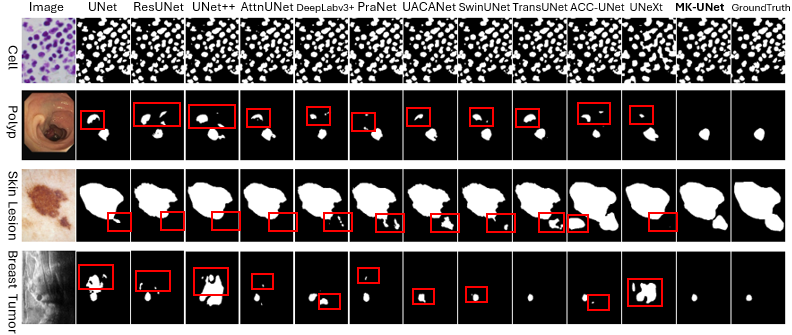
\includegraphics[width=0.95\textwidth]{sections/imgs/qualitative_results.png}
\vspace{-.2cm}
\caption{Qualitative results of our MK-UNet and SOTA methods. The incorrect segmented regions by different methods are highlighted using the red rectangular box.} 
\label{fig:qualitative}
\vspace{-.2cm}
\end{figure*}

\begin{table*}[t]
%\vspace{-.2cm}
\begin{center}
    %{\small{
    \begin{adjustbox}{width=0.75\textwidth}
\begin{tabular}{c|r|r|r|r|r|r|r|r}
\toprule
%\multicolumn{3}{c}{Components} & \multicolumn{2}{c}{\#FLOPs(G)} & \multicolumn{1}{c}{\#Params} & \multicolumn{1}{r}{Avg}  \\
Network     & \#Params & \#FLOPs & BUSI & Clinic & Colon & ISIC18 & DSB18 & EM                    \\
\midrule
Baseline UNeXt          & 1.47M & 0.57G & 74.71 &  90.20 & 83.84 &  87.78 & 86.01 & 93.81    \\
Redesigned Mobile UNet          & 0.271M     & 0.230G     & 72.41  & 90.90 & 84.15 & 87.20 & 90.52 & 94.87  \\
MKIR          & 0.306M    & 0.300G     & 74.74 & 92.63 & 86.46 & 88.22 & 92.40 & 95.31         \\
MKIR + GAG          & 0.310M     & 0.311G    & 74.98  & 91.97 & 86.56 & 88.34 & 92.67 & 95.48     \\
MKIR + MKIRA         & 0.311M    & 0.303G    &  76.61 & 92.64 & 89.40 &  88.56 & 92.64 & 95.37     \\
\textbf{MKIR + GAG + MKIRA (Ours)}        & 0.316M    & 0.314G    & \textbf{78.04} & \textbf{93.48} & \textbf{90.01} & \textbf{88.64} & \textbf{92.71} & \textbf{95.52}       \\
\bottomrule 
\end{tabular}
%}}
\end{adjustbox}
\end{center}
\vspace{-0.5cm}
\caption{Effect of different components of MK-UNet with \#channels = $[16,32,64,96,160]$ and $[1,3,5]$ kernels. UNeXt has \#channels = $[16,32,128,160,256]$. We design Mobile UNet following the structure of UNeXt network. However, we use the \#channels = $[16,32,64,96,160]$ and kernel size of $[3]$ with the original inverted residual block (IRB) in the Mobile UNet. We report the DICE scores (\%) averaging over five runs. Best results are shown in \textbf{bold}.}
\vspace{-0.4cm}
\label{tab:ablation_components}
\end{table*}


\begin{table*}[t]
%\vspace{-0.2cm}
%\vspace{-0.3cm}
\centering 
    {%\small{
\begin{adjustbox}{width=0.8\textwidth}
{\begin{tabular}{crrr|crrr}
\toprule
Convolution kernels & \#Params(M) & FLOPs(G) & DICE & Convolution kernels & \#Params(M) & FLOPs(G) & DICE\\
\midrule
$1\times1$           & 0.272 & 0.220 & 70.83 & $5\times5$           & 0.299 & 0.276 & 76.81 \\
$1\times1, 1\times1$         & 0.275 & 0.229 & 71.11 & $1\times1, 5\times5$         & 0.303 & 0.286 & 77.05 \\
$3\times3$           & 0.281 & 0.239 & 76.42 & $3\times3, 3\times3, 3\times3$       & 0.306 & 0.295 & 76.86 \\
$1\times1, 3\times3$         & 0.284 & 0.248 & 76.81 & $3\times3, 5\times5$         & 0.312 & 0.304 & 77.62 \\
$1\times1, 1\times1, 3\times3$       & 0.288 & 0.257 & 77.08 & \textbf{1$\times$1, 3$\times$3, 5$\times$5}       & 0.316 & 0.314 & \textbf{78.04} \\
$3\times3, 3\times3$         & 0.294 & 0.267 & 76.83 & $5\times5, 5\times5$         & 0.331 & 0.342 & 77.88 \\
$1\times1, 3\times3, 3\times3$       & 0.297 & 0.276 & 77.26 & $5\times5, 5\times5, 5\times5$       & 0.362 & 0.408 & 77.80 \\
%$3\times3, 5\times5, 7\times7$       & 0.371 & 0.426 & 77.63 \\
\bottomrule
\end{tabular}}
\end{adjustbox}
}%}
\vspace{-0.2cm}
\caption{Effect of multiple kernels in the depth-wise convolution of MKDC on BUSI dataset. The results for kernels beyond $7\times7$ are not reported as the performance does not scale proportionally with the computational cost of larger kernels. We use the MK-UNet network with \#channels= $[16,32,64,96,160]$ for these experiments and report the FLOPs for $256\times256$ inputs. We report the DICE scores (\%) averaging over five runs. Best results are highlighted in \textbf{bold}.}
\label{tab:multi_kernels}
\vspace{-0.2cm}
\end{table*}


\begin{table*}[t]
%\vspace{-.2cm}
  \centering
    %{\small{
    \begin{adjustbox}{width=0.65\textwidth}
\begin{tabular}{c|r|r|r|r|r|r|r|r}
\toprule
%\multicolumn{3}{c}{Components} & \multicolumn{2}{c}{\#FLOPs(G)} & \multicolumn{1}{c}{\#Params} & \multicolumn{1}{r}{Avg}  \\
Blocks     & \#Params & \#FLOPs & BUSI & Clinic & Colon & ISIC18 & DSB18 & EM                    \\
\midrule
IRB          & 0.271M     & 0.230G     & 72.41  & 90.90 & 84.15 & 87.20 & 90.52 & 94.87  \\
MKIR (\textbf{Ours})         & 0.306M    & 0.300G     & \textbf{74.74} & \textbf{92.63} & \textbf{86.46} & \textbf{88.22} & \textbf{92.40} & \textbf{95.31}         \\
\bottomrule 
\end{tabular}
%}}
\end{adjustbox}
\vspace{-0.2cm}
\caption{Original Inverted Residual Block (IRB) \cite{sandler2018mobilenetv2} vs our Multi-Kernel Inverted Residual (MKIR) with \#channels = $[16,32,64,96,160]$. We use the kernel size of $[3]$ and $[1,3,5]$ for IRB and MKIR, respectively. We report the DICE scores (\%) averaging over five runs. Best results are shown in \textbf{bold}.}
\vspace{-0.2cm}
\label{tab:ablation_irb_vs_mkir}
\end{table*}

\begin{table*}[!h]
%\vspace{-.2cm}
\begin{center}
    %{\small{
    \begin{adjustbox}{width=0.7\textwidth}
\begin{tabular}{c|c|r|r|r|r|r|r|r|r}
\toprule
%\multicolumn{3}{c}{Components} & \multicolumn{2}{c}{\#FLOPs(G)} & \multicolumn{1}{c}{\#Params} & \multicolumn{1}{r}{Avg}  \\
Encoder  & Decoder   & \#Params & \#FLOPs & BUSI & Clinic & Colon & ISIC18 & DSB18 & EM                    \\
\midrule
MKIRA & MKIRA         & 0.321M    & 0.346G    &  77.28 & 92.81 & 89.63 &  88.61 & 92.65 & 95.43     \\
(\textbf{Ours}) MKIR & MKIRA        & 0.316M    & 0.314G    & \textbf{78.04} & \textbf{93.48} & \textbf{90.01} & \textbf{88.64} & \textbf{92.71} & \textbf{95.52}       \\
\bottomrule 
\end{tabular}
%}}
\end{adjustbox}
\vspace{-0.2cm}
\caption{Effect of MKIRA in the encoder and decoder of MK-UNet with \#channels = $[16,32,64,96,160]$ and $[1,3,5]$ kernels. We report the DICE scores (\%) averaging over five runs. Best results are shown in bold.}
%\vspace{-0.3cm}
\label{tab:ablation_mkir_vs_mkira_encoder}
\end{center}
\vspace{-0.5cm}
\end{table*}

\subsection{Qualitative results}
\label{ssec:qualitative_results}

In Figure \ref{fig:qualitative}, we report the segmentation maps of breast tumors, skin lesions, polyps, and cell segmentation for representative test images. In breast tumor segmentation, UNet, UNet++, and UNeXt show greater false segmentation, while TransUNet and our MK-UNet produce near-perfect segmentation maps. Similarly, in skin lesion segmentation, UNet, ResUNet, UNet++, AttnUNet, DeepLabV3+, PraNet, SwinuNet, and UNeXt miss part of the lesion (in red rectangular box). However, UACANet, TransUNet, ACC-UNet, and our MK-UNet can segment that challenging region well. Our MK-UNet can also segment the polyp correctly, while all other methods incorrectly segment another region as a polyp. In general, our MK-UNet produces the best overlapping segmentation map in all four tasks. The reason behind this well-rounded performance by our MK-UNet with a very low computational budget is the use of multi-kernel depth-wise convolutions along with gated and local attention mechanisms.



%\vspace{-0.4cm}
\section{Ablation Study}
\label{sec:ablation_study}
This section describes three critical ablation studies. More ablation results are given in the Appendix.
%\vspace{-0.2cm}
\subsection{Effect of different components}
\label{ssec:components}
Table \ref{tab:ablation_components} presents the performance of various configurations within the MK-UNet network across six medical image segmentation datasets, highlighting the impact of integrating different components like MKIR, GAG, and MKIRA. The comparison spans models from UNeXt to the advanced MKIR + GAG + MKIRA variant, revealing a progressive improvement in the DICE scores with the addition of each component. Notably, the multi-kernel trick, implemented through MKIR (in the encoder) and MKIRA (in the decoder) blocks, is the most critical component for improving the segmentation accuracy, increasing the DICE score from 72.41\% to 76.61\% on the BUSI dataset. This indicates the significant contribution of the multi-kernel approach to feature extraction and refinement. However, when we integrate all proposed modules (MKIR + GAG + MKIRA), our model achieves the highest overall DICE score of 78.04\% on the same dataset, with minimal computational resources (0.316M \#Params and 0.314G \#FLOPs). This exhibits the efficacy of combining multi-kernel convolution with attention mechanisms within MK-UNet.%, while proving its efficiency and effectiveness in handling complex medical imaging tasks with a significantly low computational footprint. 


%\vspace{-0.4cm}
\subsection{Effect of multiple kernels}
\label{ssec:multiple_kernels}
Table \ref{tab:multi_kernels} evaluates the influence of different convolutional kernel combinations on the performance of MKDC within the MK-UNet network, specifically for the BUSI dataset. By experimenting with a variety of kernel sizes ranging from $1$ to $3,5,7$, it becomes evident that a mix of $1,3,5$ kernels stands out by achieving the best DICE score of 78.04\% with a moderate increase in computational resources (0.316M \#Params and 0.314G \#FLOPs). This finding highlights the effectiveness of a multi-scale kernel approach in capturing diverse feature representations, thus significantly improving segmentation accuracy without a substantial rise in computational demands. Drawing from these empirical findings, we opt for the kernel combination of $[1,3,5]$ across all our experiments.


\subsection{Effectiveness of our MKIR over IRB \cite{sandler2018mobilenetv2}}
\label{app:irb_mkir}

Table \ref{tab:ablation_irb_vs_mkir} reports the results of the original IRB of MobileNetv2 \cite{sandler2018mobilenetv2} and our proposed MKIR block. It can be concluded from the table that our MKIR significantly outperforms (up to 2.33\%) IRB in all the datasets with only an additional 0.035M \#Params and 0.07G \#FLOPs. The use of lightweight convolutions with multiple kernels contributes to these performance improvements with nominal additional computational resources.     



\subsection{Effectiveness of MKIR vs. MKIRA in Encoder}
\label{assec:mkir_mkira}
Table \ref{tab:ablation_mkir_vs_mkira_encoder} demonstrates that employing MKIR in the encoder and MKIRA in the decoder yields superior performance across all datasets. Specifically, this configuration achieves the best average DICE scores of 78.04\% (BUSI), 93.48\% (Clinic), 90.01\% (Colon), 88.64\% (ISIC18), 92.71\% (DSB18), and 95.52\% (EM). The MKIR block in the encoder effectively extracts complex features by leveraging multiple kernels to capture a diverse range of spatial patterns and global contexts without the need for localized attention, which is more computationally intensive. Since the encoder primarily focuses on feature extraction, this design helps preserve critical details while maintaining lightweightness. In contrast, localized attention is crucial in the decoder to facilitate precise reconstruction. The MKIRA in the decoder attends to key spatial regions, enabling effective feature refinement. This complementary setup leads to an optimal balance between performance and computational cost, as evidenced by the superior results achieved with only 0.316M \#Params and 0.314G \#FLOPs.


\section{Conclusion}
\label{sec:conclusion}
In this paper, we have presented MK-UNet, a significant advancement in the realm of medical image segmentation. MK-UNet addresses the long-standing challenge of balancing high segmentation accuracy with computational efficiency. By utilizing depth-wise convolution and multi-kernel processing, MK-UNet outperforms models like TransUNet and UNeXt with a fraction of their computational overhead (nearly 333$\times$ lower \#Params and 123$\times$ less complexity than TransUNet, and 4.7$\times$ fewer \#Params compared to UNeXt). This significant reduction in computational resources, coupled with improved performance, makes MK-UNet an optimal choice for deployment in environments where computational resources are limited, such as in point-of-care devices. 

The current evaluations of our proposed MK-UNet architecture are limited to binary medical segmentation tasks. In the future, we will extend experiments on multi-class and 3D segmentation tasks.  


\section*{Acknowledgments}
This work is supported in part by the NSF grant CNS 2007284, and in part by the iMAGiNE Consortium (https://imagine.utexas.edu/).
\vspace{-0.2cm}

{
    \small
    \bibliographystyle{ieeenat_fullname}
    \bibliography{main}
}

\clearpage
\setcounter{page}{1}
\maketitlesupplementary



\subsection{Analysis of the number of channels}
\label{assec:number_of_channels}
We conduct an ablation study with the different number of channel dimensions in different stages of the network to show the scalability of our network.
Table \ref{tab:ablation_channels} reports the results of this set of experiments. The progression from MK-UNet-T to MK-UNet-L in Table \ref{tab:ablation_channels} demonstrates a clear positive correlation between model complexity and performance. Starting with MK-UNet-T's minimal resource use (0.027M \#Params, 0.062G \#FLOPs) yielding a 75.64\% DICE score on BUSI, the score increases to 78.04\% with MK-UNet's moderate complexity (0.316M \#Params, 0.314G \#FLOPs), and peaks at 79.02\% with MK-UNet-L's higher resource demand (3.76M \#Params, 3.19G \#FLOPs). This trend of increasing DICE score with model complexity is consistent across datasets.



\begin{table*}[!b]
%\vspace{-0.5cm}
\begin{center}
    %{\small{
    \begin{adjustbox}{width=0.9\textwidth}
\begin{tabular}{c|r|r|r|r|r|r|r|r|r|r|r|r|r|r}
\toprule
Network     & C1    & C2 & C3 & C4 & C5  & \#Params & \#FLOPs & BUSI & Clinic & Colon & ISIC18 & DSB18 & EM                  \\
\midrule
MK-UNet-T           & 4  & 8 & 16  &  24 & 32     &  0.027M  & 0.062G & 75.64 & 91.26 &  85.03 & 88.19 & 92.38 & 94.69 \\
MK-UNet-S          & 8  & 16  & 32   & 48 & 80     &  0.093M & 0.125G & 77.26 & 92.31 & 88.78 & 88.57 & 92.45 & 95.22 \\
MK-UNet          & 16 & 32 & 64 & 96   & 160     & 0.316M & 0.314G &  78.04 & 93.48 &  90.01 & 88.74 & 92.71 & 95.52 \\
MK-UNet-M          & 32  & 64  & 128  &  192   & 320    & 1.15M  & 0.951G &  78.27 & 93.67 & 90.27 & 89.08 & 92.74 & 95.62 \\
MK-UNet-L          & 64  & 128  & 256 & 384  & 512    & 3.76M & 3.19G &  79.02 & 93.85 & 91.82 & 89.25 & 92.80 & 95.67 \\
\bottomrule 
\end{tabular}
%}}
\end{adjustbox}
%\vspace{-0.3cm}
\caption{Analysis of the number of channels on different datasets. \#FLOPs are reported for $256\times256$ inputs. We report the DICE scores (\%) averaging over five runs, thus having 1-4\% standard deviations.}
%\vspace{-0.8cm}
\label{tab:ablation_channels}
\end{center}
\end{table*}


\subsection{Effectiveness of our Grouped Attention Gate (GAG) over Attention Gate (AG) \cite{oktay2018attention}}
\label{assec:ag_gag}

Table \ref{tab:ablation_ag_vs_gag} reports the results of the original AG of Attention UNet \cite{oktay2018attention} and our proposed GAG block. It can be seen from the table that our GAG surpasses AG in all datasets with 0.01M fewer \#Params and 0.06G less \#FLOPs. The use of group convolutions with a relatively larger kernel ($3$) contributes to these performance improvements with less computational costs.



\begin{table*}[!b]
%\vspace{-.2cm}
\centering    %{\small{
    \begin{adjustbox}{width=0.7\textwidth}
\begin{tabular}{c|r|r|r|r|r|r|r|r}
\toprule
%\multicolumn{3}{c}{Components} & \multicolumn{2}{c}{\#FLOPs(G)} & \multicolumn{1}{c}{\#Params} & \multicolumn{1}{r}{Avg}  \\
Blocks     & \#Params & \#FLOPs & BUSI & Clinic & Colon & ISIC18 & DSB18 & EM                    \\
\midrule
AG          & 0.326M     & 0.320G     & 77.61  & 93.02 & 89.78 & 88.38 & 92.48 & 95.31  \\
GAG (\textbf{Ours})         & 0.316M    & 0.314G     & \textbf{78.04} & \textbf{93.48} & \textbf{90.01} & \textbf{88.64} & \textbf{92.71} & \textbf{95.52}         \\
\bottomrule 
\end{tabular}
%}}
\end{adjustbox}
%\vspace{-0.2cm}
\caption{Original Attention Gate (AG) \cite{sandler2018mobilenetv2} vs our Grouped Attention Gate (GAG) with \#channels = $[16,32,64,96,160]$ in MK-UNet. We use the kernel size of $3$ for GAG. We report the DICE scores (\%) averaging over five runs. Best results are shown in bold.}
\vspace{-0.4cm}
\label{tab:ablation_ag_vs_gag}
\end{table*}


%%%%%%%%%%%%%%%%%%%%%%%%%%%%%%%%%%%%%%%%%%%%%%%%%%%%%%%%%%%%

\end{document}
